\documentclass[a4paper,11pt,cours]{nsi} % COMPILE WITH DRAFT
\geometry{margin=2cm}

\begin{document}

\setcounter{chapter}{3} % 1 de moins que le num de chapitre

\chapter{Probabilités conditionnelles}



\setlength{\columnseprule}{0.5pt}
\setlength{\columnsep}{1cm}
%\creativecommonsfooter  %Pour marquer le doc


\section{Exemple d'introduction}
Un laboratoire pharmaceutique a réalisé des tests sur 800 patients atteints d'une maladie. Certains sont traités avec le médicament A, d'autres avec le médicament B.\\
Le tableau suivant présente les résultats de l'étude :
\begin{center}
	\begin{tabular}{|l|c|c|c|}
		\hline
		& Médicament A & Médicament B & Total\\
		\hline
		Guéri & 383 & 291 & 674\\
		\hline
		Non guéri & 72 & 54 & 126\\
		\hline
		Total & 455 & 345 & 800\\
		\hline
	\end{tabular}
\end{center}
\begin{enumerate}
	\item 	On choisit au hasard un patient et on considère les évènements suivants:\\
	A : « Le patient a pris le médicament A »\\
	G : « Le patient est guéri ».\\
	
	On a alors :
	\begin{enumerate}[label=\textbullet]
		\item 	La probabilité qu'un patient soit traité avec le médicament A est : \\[0.5em]
		\carreauxseyes{16}{1.6}
		\item 	La probabilité qu'un patient soit guéri est : \\[0.5em]
		\carreauxseyes{16}{1.6}
		\item	La probabilité qu'un patient soit guéri et qu'il soit traité avec le médicament A est : \\[0.5em]
		\carreauxseyes{16}{1.6}
		\item	La probabilité qu'un patient ne soit pas guéri et qu'il soit traité avec le médicament A est : \\[0.5em]
		\carreauxseyes{16}{1.6}
	\end{enumerate}
	
	\item 	On choisi maintenant au hasard un \textbf{patient guéri}.
	\begin{center}
		\begin{tabular}{|l|c|c|c|}
			\hline
			& Médicament A & \cellcolor{UGLiOrange}Médicament B & Total\\
			\hline
			\rowcolor{UGLiBlue}Guéri & 383 & \cellcolor{UGLiPurple}291 & 674\\
			\hline
			Non guéri & 72 & \cellcolor{UGLiOrange}54 & 126\\
			\hline
			Total & 455 & \cellcolor{UGLiOrange}345 & 800\\
			\hline
		\end{tabular}
	\end{center}
	\begin{enumerate}[label=\textbullet]
		\item 	La probabilité que le patient ait pris le médicament A \textcolor{UGLiBlue}{\textbf{sachant qu'il est guéri} } se note $P_G(A)$. Elle est égale à :\\[0.5em]
		\carreauxseyes{16}{1.6}
		\item 	La probabilité que le soit guéri \textcolor{UGLiOrange}{\textbf{sachant qu'il a pris le médicament B}} se note $P_B(G)$. Elle est égale à : \\[0.5em]
		\carreauxseyes{16}{1.6}
	\end{enumerate}
\end{enumerate}

\vspace{1cm}

Dans tout le cours, on considère une expérience aléatoire d'univers fini $\Omega$ et $P$ une probabilité sur $\Omega$. $A$, $B$ et $C$ sont des évènements de $\Omega$  tels que $P(A) \neq 0$.

\section{Notion de probabilité conditionnelle}
\subsection{Probabilité de l'évènement B sachant que A est réalisé}
\begin{definition}[ ]
	La \textbf{probabilité conditionnelle} que l'évènement $B$ se réalise sachant que l'évènement $A$ est réalisé est le nombre 
	$$P_A(B)=\dfrac{P(A\cap B)}{P(A)}$$
	$P_A(B)$ se lit « \textit{probabilité de $B$ sachant $A$} ».
\end{definition}

\begin{propriete}[ ]
	La fonction $P_A$, définie sur $\Omega$ est une loi de probabilité appelée \textbf{loi de probabilité conditionnelle sachant $A$}.
\end{propriete}

%\newpage
\begin{demonstration}
	Pour que $P_A$ soit une loi de probabilité sur $\Omega$, elle doit vérifier :
	\begin{enumerate}[label=\textbullet]
		\item 	$P_A(\Omega)=1 \quad$ et $\quad P_A(\varnothing)=0$ ; 
		\item 	$0\leqslant P_A(B) \leqslant 1$ ;
		\item	Si $B$ et $C$ sont disjoints, $\quad P_A(B\cup C)=P_A(B)+P_A(C)$.
	\end{enumerate}
	Vérifions chacun des ces points :
	\begin{enumerate}
		\item	
		
		
		\begin{multicols}{2}
			\begin{tabbing}
				$P_A(\Omega)$ \=	$=\dfrac{P(A\cap \Omega)}{P(A)}$ \=\\[0.5em]
				\>	$=\dfrac{P(A)}{P(A)}$	\>car $A$ est inclus dans $\Omega$\\[0.5em]
				\>	$=1$
			\end{tabbing}
		
			\begin{tabbing}
				$P_A(\varnothing)$ \=	$=\dfrac{P(A\cap \varnothing)}{P(A)}$ \\[0.5em]
				\>	$=\dfrac{P(\varnothing)}{P(A)}$	\\[0.5em]
				\>	$=0$
			\end{tabbing}
		\end{multicols} 
		
		
		\item 	$A \cap B$ est inclus dans $A$ donc $0\leqslant P(A\cap B) \leqslant P(A)$.\\[0.5em]
			Ainsi $\quad 0 \leqslant	\dfrac{P(A \cap B)}{P(A)} \leqslant	\dfrac{P(A)}{P(A)} \quad$ c'est-à-dire $\quad 0\leqslant P_A(B) \leqslant 1$.
		\item	Soient $B$ et $C$ deux évènements disjoints.
		\begin{center}
			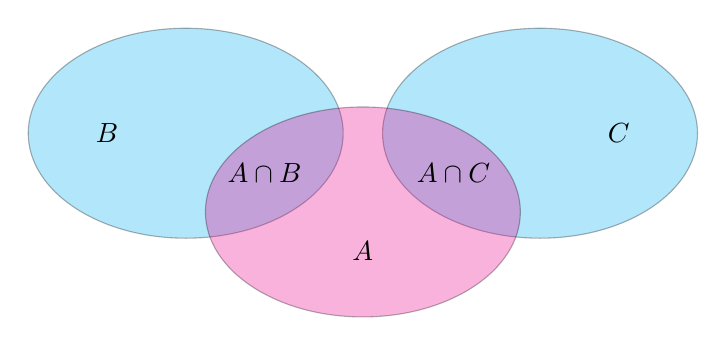
\begin{tikzpicture}
				\draw[fill = cyan,opacity = .3](0,0) ellipse (2 and 4/3);
				\draw[fill = cyan,opacity = .3](4.5,0) ellipse (2 and 4/3);
				\draw[fill = magenta,opacity = .3](2.25,-1) ellipse (2 and 4/3);
				\draw (-1,0) node{$B$};
				\draw (5.5,0) node{$C$};
				\draw (2.25,-1.5) node{$A$};
				\draw (1,-0.5) node{$A\cap B$};
				\draw (3.4,-0.5) node{$A\cap C$};
			\end{tikzpicture}
		\end{center}
		\begin{tabbing}
			$P_A(B\cup C)$ \= $=\dfrac{P(A\cap (B \cup C))}{P(A)}$\\[0.5em]
			\>	$=\dfrac{P((A\cap B)\cup (A\cap C))}{P(A)}$\\[0.5em]
			\>	$=\dfrac{P(A\cap B)+P(A\cap C)}{P(A)}\quad$ car $A\cap B$ et $A\cap C$ sont disjoints\\[0.5em]
			\>	$=\dfrac{P(A \cap B)}{P(A)}+\dfrac{P(A\cap C)}{P(A)}$\\[0.5em]
			\>	$=P_A(B)+P_A(C)$
		\end{tabbing}
	\end{enumerate}
\end{demonstration}

\begin{propriete}[ ]
	Si $A$ et $B$ sont deux évènements de probabilité non nulle, alors 
	$$P(A\cap B)=P(A)\times P_A(B)=P(B) \times P_B(A)$$
\end{propriete}

\begin{exercice}[]
	Dans un classe de première, 55 \% des élèves sont des filles et 40 \% des élèves sont des filles demi-pensionnaires.\\
	On choisit au hasard un élève au hasard dans cette classe. Quelle est la probabilité que cet élève soit demi-pensionnaire sachant que c'est une fille ?\\[.5em]
	\carreauxseyes{16}{2.4}\\
	\carreauxseyes{16}{8}
\end{exercice}

\subsection{Utilisation de tableaux}
Les tableaux à double entrée permettent un présentation claire de certaines expériences aléatoires et facilitent le calcul des probabilités conditionnelles.

\begin{center}
	\begin{tabular}{|c|c|c|c|}
		\hline
		 \rowcolor{UGLiOrange}& $B$ & $\overline{B}$ & Total\\
		 \hline
		 \cellcolor{UGLiOrange}$A$ & $P(A\cap B) $ & $P(A \cap \overline{B})$ & $P(A)$\\
		 \hline
		 \cellcolor{UGLiOrange}$\overline{A}$ & $P(\overline{A}\cap B)$ & $P(\overline{A}\cap \overline{B})$ & $P(\overline{A})$\\
		 \hline
		 \cellcolor{UGLiOrange}Total & $P(B)$ & $P(\overline{B})$ & 1\\
		 \hline
	\end{tabular}
\end{center}

\begin{exercice}[ ]
	Un club sportif rassemble 180 membres répartis en junior et seniors. On compte 135 seniors dont 81 hommes. Il y a 27 garçons parmi les juniors.\\
	En choisissant une femme au hasard, calculer la probabilité d'avoir une juniore.	
\end{exercice}

\begin{methode}[ ]
	\begin{enumerate}
		\item 	On définit les évènements :
		\begin{enumerate}[label=\textbullet]
			\item 	H : La personne choisie au hasard est un homme ;
			\item 	J : La personne choisie au hasard appartient à la catégorie junior.
		\end{enumerate}
		\item 	On construit un tableau à double entrée que l'on complète à l'aide des informations de l'énoncé.
		\begin{center}
			\begin{tabular}{|c|p{4cm}|p{4cm}|p{4cm}|}
				\hline
				\rowcolor{UGLiOrange}  & \makebox[\linewidth][c]{$J$} & \makebox[\linewidth][c]{$\overline{J}$} & \makebox[\linewidth][c]{Total}\\
				\hline
				\cellcolor{UGLiOrange} & & & \\
				\cellcolor{UGLiOrange} $H$ & & & \\
				\cellcolor{UGLiOrange} & & & \\
				\hline
				\cellcolor{UGLiOrange} & & & \\
				\cellcolor{UGLiOrange} $\overline{H}$ & & & \\
				\cellcolor{UGLiOrange} & & & \\
				\hline
				\cellcolor{UGLiOrange} & & & \\
				\cellcolor{UGLiOrange} Total & & & \\
				\cellcolor{UGLiOrange} & & & \\
				\hline
			\end{tabular}
		\end{center}
		\item	On détermine $P_{\overline{H}}(J)$ en calculant $\dfrac{P(\overline{H}\cap J)}{P(\overline{H})}$.\\
		\carreauxseyes{16}{3.2}
	\end{enumerate}
\end{methode}

\section{Formule des probabilités totales}
\subsection{Arbre pondéré}

\begin{propriete}[s (admises)]
	\begin{enumerate}
		\item 	La somme des probabilités des branches issues d'un nœud est égale à 1.
		\item 	La probabilité de l'évènement à l'extrémité d'un chemin est égale au produit des probabilités des branches composant ce chemin.
		\item	La probabilité d'un évènement est égale à la somme des probabilités des chemins conduisant à cet évènement.
	\end{enumerate}

\begin{center}
	
	{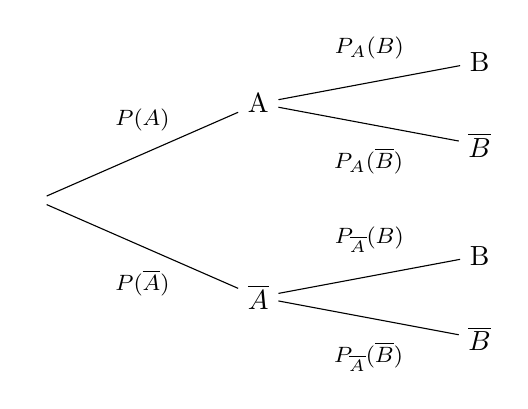
\begin{tikzpicture}[grow = right,level distance=8em,level 1/.style={sibling distance=7em},
			level 2/.style={sibling distance=3em}]
			\node{}
			child
			{
				node {$\overline{A}$} 
				child 
				{
					node {$\overline{B}$} 
					edge from parent node[below=.5em] {\footnotesize$P_{\overline{A}}(\overline{B})$}
				} 
				child 
				{
					node {B}
					edge from parent node[above=.5em] {\footnotesize$P_{\overline{A}}(B)$}
				}
				edge from parent node[below=.5em] {\footnotesize$P(\overline{A})$}
			}
			child
			{
				node {A} 
				child 
				{
					node {$\overline{B}$} 
					edge from parent node[below=.5em] {\footnotesize$P_A(\overline{B})$}
				}
				child 
				{
					node {B}
					edge from parent node[above=.5em] {\footnotesize$P_A(B)$}
				}
				edge from parent node[above=.5em] {\footnotesize$P(A)$}
			};
	\end{tikzpicture}}
\end{center}
\end{propriete}

\begin{exemple}[ ]
	On considère l'arbre pondéré ci-dessous :
	\begin{center}
		
		{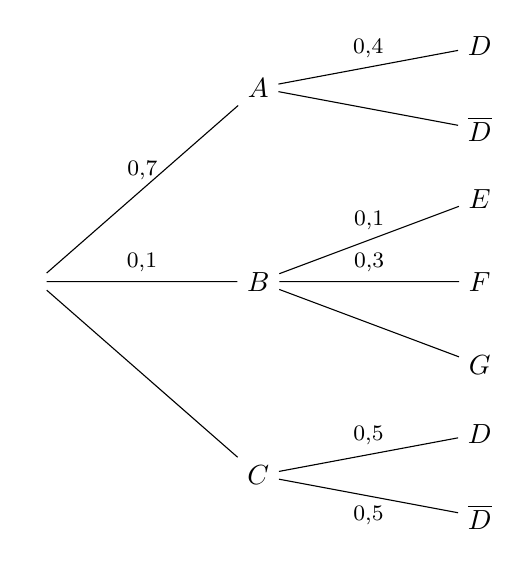
\begin{tikzpicture}[grow = right,level distance=8em,level 1/.style={sibling distance=7em},
				level 2/.style={sibling distance=3em}]
				\node{}
				child
				{
					node {$C$} 
					child 
					{
						node {$\overline{D}$} 
						edge from parent node[below] {\footnotesize 0,5}
					} 
					child 
					{
						node {$D$}
						edge from parent node[above] {\footnotesize 0,5}
					}
					edge from parent node[below=.5em] {}
				}
				child
				{
					node {$B$} 
					child 
					{
						node {$G$} 
						edge from parent node[below=.5em] {}
					}
					child 
					{
						node {$F$}
						edge from parent node[above] {\footnotesize 0,3}
					}
					child 
					{
						node {$E$}
						edge from parent node[above] {\footnotesize 0,1}
					}
					edge from parent node[above] {\footnotesize 0,1}
				}
				child
				{
					node {$A$} 
					child 
					{
						node {$\overline{D}$} 
						edge from parent node[below=.5em] {}
					}
					child 
					{
						node {$D$}
						edge from parent node[above] {\footnotesize 0,4}
					}
					edge from parent node[above] {\footnotesize 0,7}
				};
		\end{tikzpicture}}
	\end{center}
\begin{enumerate}[label=\textbullet]
	\item 	D'après la première propriété : \\
	$P(A)+P(B)+P(C)=1,\quad P_A(D)+P_A(\overline{D})=1 \quad$ et $\quad P_B(E)+P_B(F)+P_B(G)=1$\\[0.5em]
	\carreauxseyes{16}{3.2}
	\item 	D'après la deuxième propriété, $\quad P(A\cap D)=P(A)\times P_A(D)\quad$ d'où :\\[0.5em]
	\carreauxseyes{16}{1.6}
	\item	D'après la troisième propriété, $\quad P(D) = P(A\cap D)+P(C \cap D)$ d'où :\\[0.5em]
	\carreauxseyes{16}{3.2}
\end{enumerate}
\end{exemple}

\begin{exercice}[ : Calculer des probabilités conditionnelles à l'aide d'un arbre]
	Lors d’une épidémie chez des bovins, on s’est aperçu que si la maladie est
	diagnostiquée suffisamment tôt chez un animal, on peut le guérir ; sinon la maladie
	est mortelle.\\
	Un test est mis au point et essayé sur un échantillon d’animaux dont 2 \% est porteur
	de la maladie.
	On obtient les résultats suivants :
	\begin{enumerate}[label=\textbullet]
		\item 	sachant qu’un animal est porteur de la maladie, le test est positif dans 85 \% des
		cas ;
		\item 	sachant qu’un animal est sain, le test est négatif dans 95 \% des cas.	
	\end{enumerate}
	On note les événements :
	\begin{enumerate}[label=\textbullet]
		\item 	$M$ : « Être porteur de la maladie »
		\item 	$T$ : « Avoir un test positif ».
	\end{enumerate}

\begin{enumerate}
	\item 	Construire un arbre pondéré traduisant les données de l'énoncé.
	\item 	Un animal est choisi au hasard. Quelle est la probabilité que son test soit positif ?
	\item	Si le test du bovin est positif, quelle est la probabilité qu'il soit malade ?
\end{enumerate}
\carreauxseyes{16}{18.4}
\end{exercice}

\subsection{Probabilités totales}
\begin{definition}[ ]
	\dleft{10.5cm}{
	On considère un événement $A$ ainsi que les $n$ événements non vides $A_1,A_2,...,A_n$ tels que :
	\begin{enumerate}[label=\textbullet]
		\item 	pour tous entiers distincts $i$ et $j$ compris entre $1$ et $n$, $A_i$ et $A_j$ sont \textbf{incompatibles} : $A_i\cap A_j= \emptyset$ ;
		\item 	$A_1\cup A_2 \cup ... \cup A_n=A$
	\end{enumerate}
	}{\includegraphics[width=4cm]{partition1}}

	On dit alors que la famille des événements $\left(A_k\right)_{1\leqslant k \leqslant n}$ forme une \textbf{partition} de $A$.
	
\end{definition}

\begin{remarque}[ ]
	$A$ et $\overline{A}$ forment toujours une partition de $\Omega$.
\end{remarque}

\begin{propriete}[ : formule des probabilités totales]
	On considère une expérience aléatoire d'univers $\Omega$ et un événement $B$. On note $A_1,A_2,...,A_n$, $n$ événements non vides formant une partition de l'univers $\Omega$.\\
	On a alors : 
	$$\quad P(B)=P(A_1\cap B)+P(A_2\cap B)+...+P(A_n\cap B).$$
	Ce que l'on peut également écrire :
	$$P(B)=P(A_1)\times P_{A_1}(B)+P(A_2)\times P_{A_2}(B)+...+P(A_n)\times P_{A_n}(B).$$
\end{propriete}



\begin{demonstration}
		
	\dleft{11cm}{
		\begin{tabbing}
			$P(B)$ \=$=P(B\cap \Omega)$\\
			\>	$=P\left(B\cap(A_1\cup A_2 \cup ... \cup A_n)\right)$\\
			\>	$=P\left((B\cap A_1)\cup(B\cap A_2)\cup ... \cup(B\cap A_n)\right)$\\
			\>	$=P(B\cap A_1)+P(B\cap A_2)+...+P(B\cap A_n)\quad$
		\end{tabbing}
		En effet, les événements $A_i$ et $A_j$ sont incompatibles pour tous les entiers $i\neq j$ et donc les événements $B\cap A_i$ et $B\cap A_j$ le sont aussi.\\
		
	}{
		\includegraphics[width=4cm]{demonstration_proba_totales}
	}
\end{demonstration}

\begin{remarque}[ ]
	On a vu en seconde que : $\quad P(B)=P(A\cap B)+P(\overline{A} \cap B)\quad$ où $A$ et $\overline{A}$ forment une partition de $\Omega$.\\
	La formule des probabilités totale est une généralisation de cette propriété.
\end{remarque}

\begin{exemple}[ ]
	\begin{center}
		\includegraphics[width=12cm]{exemple}
	\end{center}
Ici, $A,B$ et $C$ forment une partition de l'univers $\Omega$. On a donc :
\begin{tabbing}
	$P(D)$ \= $=P(A\cap D)+P(B\cap D)+P(C\cap D)$\\
	\>	$=P(A)\times P_A(D)+P(B)\times P_B(D)+P(C)\times P_C(D)$\\
	\>	$=0,1 \times 0,2 + 0,5 \times 0,7 + 0,4 \times 0,1$\\
	\>	$=0,41$
\end{tabbing}
\end{exemple}

\section{Indépendance}
\begin{definition}[ ]
	Soient $A$ et $B$ deux événements d'un univers $\Omega$.\\
	On dit que $A$ et $B$ sont \textbf{indépendants} lorsque $\quad P(A\cap B)=P(A)\times P(B)$.
\end{definition}

\begin{propriete}[ ]
	Soient $A$ et $B$ deux événements d'un univers $\Omega$ tels que $P(A)\neq 0$.\\
	$A$ et $B$ sont des événements indépendants si, et seulement si, $\ P_A(B)=P(B)$.
\end{propriete}

\begin{demonstration}
	$P(A)\neq 0 \quad$ donc $\quad P_A(B)=\dfrac{P(A\cap B)}{P(A)}$.\\
	\textbf{Sens direct :}\\
	Supposons que $A$ et $B$ sont des événements indépendants.\\
	On a alors : $\quad P(A\cap B)=P(A)\times P(B)$.\\[0.5em]
	D'où $\quad P_A(B)=\dfrac{P(A)\times P(B)}{P(A)}=P(B)$.\\[0.5em]
	\textbf{Réciproque :}\\
	Supposons que $\quad P_A(B)=P(B)$.\\
	On a donc $\quad P(A)\times P_A(B)=P(A)\times P(B)$.\\
	D'où $\quad P(A\cap B)=P(A)\times P(B)$.\\
	Ainsi on a montré que $A$ et $B$ sont indépendants.
\end{demonstration}

\begin{exemple}[ ]
	Soient $A$ et $B$ deux événements indépendants tels que $P(A)=0,8$ et $P(B)=0,35$.\\
	Alors $\quad P(A\cap B)=P(A)\times P(B)=0,8\times 0,35=0,28$.
\end{exemple}

\begin{propriete}[ ]
	Si $A$ et $B$ sont deux événements indépendants, alors $\overline{A}$ et $B$ sont aussi deux événements indépendants.
\end{propriete}

\begin{demonstration}
	En exercice \\[0.5em]
	\carreauxseyes{16}{6.4}
\end{demonstration}
\begin{exemple}[ d'application]
	Soient $A$ et $B$ deux événements tels que $P(A)=0,8$ ; $P(B)=0,35$ et $P(A\cap B)=0,28$.
	\begin{enumerate}
		\item 	Montrer que $A$ et $B$ sont indépendants.
		\item 	Déterminer $\ P(A\cup B)\ $ puis $\ P(\overline{A} \cap B)$.
	\end{enumerate}
	\begin{methode}[ ]
		\begin{enumerate}
			\item 	On compare $\ P(A)\times P(B)\ $ et $\ P(A\cap B)$ :\\
			\carreauxseyes{15.2}{1.6}
			\item 	On utilise $\ P(A\cup B)=P(A)+P(B)-P(A\cap B)\ $ et l'indépendance de $\overline{A}$ et $B$.\\
			\carreauxseyes{15.2}{3.2}
		\end{enumerate}
	\end{methode}
\end{exemple}
\begin{aretenir}
	\includegraphics[width=16.5cm]{cartementale}
\end{aretenir}


\end{document}